
% Default to the notebook output style

    


% Inherit from the specified cell style.




    
\documentclass[11pt]{article}

    
    
    \usepackage[T1]{fontenc}
    % Nicer default font (+ math font) than Computer Modern for most use cases
    \usepackage{mathpazo}

    % Basic figure setup, for now with no caption control since it's done
    % automatically by Pandoc (which extracts ![](path) syntax from Markdown).
    \usepackage{graphicx}
    % We will generate all images so they have a width \maxwidth. This means
    % that they will get their normal width if they fit onto the page, but
    % are scaled down if they would overflow the margins.
    \makeatletter
    \def\maxwidth{\ifdim\Gin@nat@width>\linewidth\linewidth
    \else\Gin@nat@width\fi}
    \makeatother
    \let\Oldincludegraphics\includegraphics
    % Set max figure width to be 80% of text width, for now hardcoded.
    \renewcommand{\includegraphics}[1]{\Oldincludegraphics[width=.8\maxwidth]{#1}}
    % Ensure that by default, figures have no caption (until we provide a
    % proper Figure object with a Caption API and a way to capture that
    % in the conversion process - todo).
    \usepackage{caption}
    \DeclareCaptionLabelFormat{nolabel}{}
    \captionsetup{labelformat=nolabel}

    \usepackage{adjustbox} % Used to constrain images to a maximum size 
    \usepackage{xcolor} % Allow colors to be defined
    \usepackage{enumerate} % Needed for markdown enumerations to work
    \usepackage{geometry} % Used to adjust the document margins
    \usepackage{amsmath} % Equations
    \usepackage{amssymb} % Equations
    \usepackage{textcomp} % defines textquotesingle
    % Hack from http://tex.stackexchange.com/a/47451/13684:
    \AtBeginDocument{%
        \def\PYZsq{\textquotesingle}% Upright quotes in Pygmentized code
    }
    \usepackage{upquote} % Upright quotes for verbatim code
    \usepackage{eurosym} % defines \euro
    \usepackage[mathletters]{ucs} % Extended unicode (utf-8) support
    \usepackage[utf8x]{inputenc} % Allow utf-8 characters in the tex document
    \usepackage{fancyvrb} % verbatim replacement that allows latex
    \usepackage{grffile} % extends the file name processing of package graphics 
                         % to support a larger range 
    % The hyperref package gives us a pdf with properly built
    % internal navigation ('pdf bookmarks' for the table of contents,
    % internal cross-reference links, web links for URLs, etc.)
    \usepackage{hyperref}
    \usepackage{longtable} % longtable support required by pandoc >1.10
    \usepackage{booktabs}  % table support for pandoc > 1.12.2
    \usepackage[inline]{enumitem} % IRkernel/repr support (it uses the enumerate* environment)
    \usepackage[normalem]{ulem} % ulem is needed to support strikethroughs (\sout)
                                % normalem makes italics be italics, not underlines
    

    
    
    % Colors for the hyperref package
    \definecolor{urlcolor}{rgb}{0,.145,.698}
    \definecolor{linkcolor}{rgb}{.71,0.21,0.01}
    \definecolor{citecolor}{rgb}{.12,.54,.11}

    % ANSI colors
    \definecolor{ansi-black}{HTML}{3E424D}
    \definecolor{ansi-black-intense}{HTML}{282C36}
    \definecolor{ansi-red}{HTML}{E75C58}
    \definecolor{ansi-red-intense}{HTML}{B22B31}
    \definecolor{ansi-green}{HTML}{00A250}
    \definecolor{ansi-green-intense}{HTML}{007427}
    \definecolor{ansi-yellow}{HTML}{DDB62B}
    \definecolor{ansi-yellow-intense}{HTML}{B27D12}
    \definecolor{ansi-blue}{HTML}{208FFB}
    \definecolor{ansi-blue-intense}{HTML}{0065CA}
    \definecolor{ansi-magenta}{HTML}{D160C4}
    \definecolor{ansi-magenta-intense}{HTML}{A03196}
    \definecolor{ansi-cyan}{HTML}{60C6C8}
    \definecolor{ansi-cyan-intense}{HTML}{258F8F}
    \definecolor{ansi-white}{HTML}{C5C1B4}
    \definecolor{ansi-white-intense}{HTML}{A1A6B2}

    % commands and environments needed by pandoc snippets
    % extracted from the output of `pandoc -s`
    \providecommand{\tightlist}{%
      \setlength{\itemsep}{0pt}\setlength{\parskip}{0pt}}
    \DefineVerbatimEnvironment{Highlighting}{Verbatim}{commandchars=\\\{\}}
    % Add ',fontsize=\small' for more characters per line
    \newenvironment{Shaded}{}{}
    \newcommand{\KeywordTok}[1]{\textcolor[rgb]{0.00,0.44,0.13}{\textbf{{#1}}}}
    \newcommand{\DataTypeTok}[1]{\textcolor[rgb]{0.56,0.13,0.00}{{#1}}}
    \newcommand{\DecValTok}[1]{\textcolor[rgb]{0.25,0.63,0.44}{{#1}}}
    \newcommand{\BaseNTok}[1]{\textcolor[rgb]{0.25,0.63,0.44}{{#1}}}
    \newcommand{\FloatTok}[1]{\textcolor[rgb]{0.25,0.63,0.44}{{#1}}}
    \newcommand{\CharTok}[1]{\textcolor[rgb]{0.25,0.44,0.63}{{#1}}}
    \newcommand{\StringTok}[1]{\textcolor[rgb]{0.25,0.44,0.63}{{#1}}}
    \newcommand{\CommentTok}[1]{\textcolor[rgb]{0.38,0.63,0.69}{\textit{{#1}}}}
    \newcommand{\OtherTok}[1]{\textcolor[rgb]{0.00,0.44,0.13}{{#1}}}
    \newcommand{\AlertTok}[1]{\textcolor[rgb]{1.00,0.00,0.00}{\textbf{{#1}}}}
    \newcommand{\FunctionTok}[1]{\textcolor[rgb]{0.02,0.16,0.49}{{#1}}}
    \newcommand{\RegionMarkerTok}[1]{{#1}}
    \newcommand{\ErrorTok}[1]{\textcolor[rgb]{1.00,0.00,0.00}{\textbf{{#1}}}}
    \newcommand{\NormalTok}[1]{{#1}}
    
    % Additional commands for more recent versions of Pandoc
    \newcommand{\ConstantTok}[1]{\textcolor[rgb]{0.53,0.00,0.00}{{#1}}}
    \newcommand{\SpecialCharTok}[1]{\textcolor[rgb]{0.25,0.44,0.63}{{#1}}}
    \newcommand{\VerbatimStringTok}[1]{\textcolor[rgb]{0.25,0.44,0.63}{{#1}}}
    \newcommand{\SpecialStringTok}[1]{\textcolor[rgb]{0.73,0.40,0.53}{{#1}}}
    \newcommand{\ImportTok}[1]{{#1}}
    \newcommand{\DocumentationTok}[1]{\textcolor[rgb]{0.73,0.13,0.13}{\textit{{#1}}}}
    \newcommand{\AnnotationTok}[1]{\textcolor[rgb]{0.38,0.63,0.69}{\textbf{\textit{{#1}}}}}
    \newcommand{\CommentVarTok}[1]{\textcolor[rgb]{0.38,0.63,0.69}{\textbf{\textit{{#1}}}}}
    \newcommand{\VariableTok}[1]{\textcolor[rgb]{0.10,0.09,0.49}{{#1}}}
    \newcommand{\ControlFlowTok}[1]{\textcolor[rgb]{0.00,0.44,0.13}{\textbf{{#1}}}}
    \newcommand{\OperatorTok}[1]{\textcolor[rgb]{0.40,0.40,0.40}{{#1}}}
    \newcommand{\BuiltInTok}[1]{{#1}}
    \newcommand{\ExtensionTok}[1]{{#1}}
    \newcommand{\PreprocessorTok}[1]{\textcolor[rgb]{0.74,0.48,0.00}{{#1}}}
    \newcommand{\AttributeTok}[1]{\textcolor[rgb]{0.49,0.56,0.16}{{#1}}}
    \newcommand{\InformationTok}[1]{\textcolor[rgb]{0.38,0.63,0.69}{\textbf{\textit{{#1}}}}}
    \newcommand{\WarningTok}[1]{\textcolor[rgb]{0.38,0.63,0.69}{\textbf{\textit{{#1}}}}}
    
    
    % Define a nice break command that doesn't care if a line doesn't already
    % exist.
    \def\br{\hspace*{\fill} \\* }
    % Math Jax compatability definitions
    \def\gt{>}
    \def\lt{<}
    % Document parameters
    \title{understandingQubits}
    
    
    

    % Pygments definitions
    
\makeatletter
\def\PY@reset{\let\PY@it=\relax \let\PY@bf=\relax%
    \let\PY@ul=\relax \let\PY@tc=\relax%
    \let\PY@bc=\relax \let\PY@ff=\relax}
\def\PY@tok#1{\csname PY@tok@#1\endcsname}
\def\PY@toks#1+{\ifx\relax#1\empty\else%
    \PY@tok{#1}\expandafter\PY@toks\fi}
\def\PY@do#1{\PY@bc{\PY@tc{\PY@ul{%
    \PY@it{\PY@bf{\PY@ff{#1}}}}}}}
\def\PY#1#2{\PY@reset\PY@toks#1+\relax+\PY@do{#2}}

\expandafter\def\csname PY@tok@w\endcsname{\def\PY@tc##1{\textcolor[rgb]{0.73,0.73,0.73}{##1}}}
\expandafter\def\csname PY@tok@c\endcsname{\let\PY@it=\textit\def\PY@tc##1{\textcolor[rgb]{0.25,0.50,0.50}{##1}}}
\expandafter\def\csname PY@tok@cp\endcsname{\def\PY@tc##1{\textcolor[rgb]{0.74,0.48,0.00}{##1}}}
\expandafter\def\csname PY@tok@k\endcsname{\let\PY@bf=\textbf\def\PY@tc##1{\textcolor[rgb]{0.00,0.50,0.00}{##1}}}
\expandafter\def\csname PY@tok@kp\endcsname{\def\PY@tc##1{\textcolor[rgb]{0.00,0.50,0.00}{##1}}}
\expandafter\def\csname PY@tok@kt\endcsname{\def\PY@tc##1{\textcolor[rgb]{0.69,0.00,0.25}{##1}}}
\expandafter\def\csname PY@tok@o\endcsname{\def\PY@tc##1{\textcolor[rgb]{0.40,0.40,0.40}{##1}}}
\expandafter\def\csname PY@tok@ow\endcsname{\let\PY@bf=\textbf\def\PY@tc##1{\textcolor[rgb]{0.67,0.13,1.00}{##1}}}
\expandafter\def\csname PY@tok@nb\endcsname{\def\PY@tc##1{\textcolor[rgb]{0.00,0.50,0.00}{##1}}}
\expandafter\def\csname PY@tok@nf\endcsname{\def\PY@tc##1{\textcolor[rgb]{0.00,0.00,1.00}{##1}}}
\expandafter\def\csname PY@tok@nc\endcsname{\let\PY@bf=\textbf\def\PY@tc##1{\textcolor[rgb]{0.00,0.00,1.00}{##1}}}
\expandafter\def\csname PY@tok@nn\endcsname{\let\PY@bf=\textbf\def\PY@tc##1{\textcolor[rgb]{0.00,0.00,1.00}{##1}}}
\expandafter\def\csname PY@tok@ne\endcsname{\let\PY@bf=\textbf\def\PY@tc##1{\textcolor[rgb]{0.82,0.25,0.23}{##1}}}
\expandafter\def\csname PY@tok@nv\endcsname{\def\PY@tc##1{\textcolor[rgb]{0.10,0.09,0.49}{##1}}}
\expandafter\def\csname PY@tok@no\endcsname{\def\PY@tc##1{\textcolor[rgb]{0.53,0.00,0.00}{##1}}}
\expandafter\def\csname PY@tok@nl\endcsname{\def\PY@tc##1{\textcolor[rgb]{0.63,0.63,0.00}{##1}}}
\expandafter\def\csname PY@tok@ni\endcsname{\let\PY@bf=\textbf\def\PY@tc##1{\textcolor[rgb]{0.60,0.60,0.60}{##1}}}
\expandafter\def\csname PY@tok@na\endcsname{\def\PY@tc##1{\textcolor[rgb]{0.49,0.56,0.16}{##1}}}
\expandafter\def\csname PY@tok@nt\endcsname{\let\PY@bf=\textbf\def\PY@tc##1{\textcolor[rgb]{0.00,0.50,0.00}{##1}}}
\expandafter\def\csname PY@tok@nd\endcsname{\def\PY@tc##1{\textcolor[rgb]{0.67,0.13,1.00}{##1}}}
\expandafter\def\csname PY@tok@s\endcsname{\def\PY@tc##1{\textcolor[rgb]{0.73,0.13,0.13}{##1}}}
\expandafter\def\csname PY@tok@sd\endcsname{\let\PY@it=\textit\def\PY@tc##1{\textcolor[rgb]{0.73,0.13,0.13}{##1}}}
\expandafter\def\csname PY@tok@si\endcsname{\let\PY@bf=\textbf\def\PY@tc##1{\textcolor[rgb]{0.73,0.40,0.53}{##1}}}
\expandafter\def\csname PY@tok@se\endcsname{\let\PY@bf=\textbf\def\PY@tc##1{\textcolor[rgb]{0.73,0.40,0.13}{##1}}}
\expandafter\def\csname PY@tok@sr\endcsname{\def\PY@tc##1{\textcolor[rgb]{0.73,0.40,0.53}{##1}}}
\expandafter\def\csname PY@tok@ss\endcsname{\def\PY@tc##1{\textcolor[rgb]{0.10,0.09,0.49}{##1}}}
\expandafter\def\csname PY@tok@sx\endcsname{\def\PY@tc##1{\textcolor[rgb]{0.00,0.50,0.00}{##1}}}
\expandafter\def\csname PY@tok@m\endcsname{\def\PY@tc##1{\textcolor[rgb]{0.40,0.40,0.40}{##1}}}
\expandafter\def\csname PY@tok@gh\endcsname{\let\PY@bf=\textbf\def\PY@tc##1{\textcolor[rgb]{0.00,0.00,0.50}{##1}}}
\expandafter\def\csname PY@tok@gu\endcsname{\let\PY@bf=\textbf\def\PY@tc##1{\textcolor[rgb]{0.50,0.00,0.50}{##1}}}
\expandafter\def\csname PY@tok@gd\endcsname{\def\PY@tc##1{\textcolor[rgb]{0.63,0.00,0.00}{##1}}}
\expandafter\def\csname PY@tok@gi\endcsname{\def\PY@tc##1{\textcolor[rgb]{0.00,0.63,0.00}{##1}}}
\expandafter\def\csname PY@tok@gr\endcsname{\def\PY@tc##1{\textcolor[rgb]{1.00,0.00,0.00}{##1}}}
\expandafter\def\csname PY@tok@ge\endcsname{\let\PY@it=\textit}
\expandafter\def\csname PY@tok@gs\endcsname{\let\PY@bf=\textbf}
\expandafter\def\csname PY@tok@gp\endcsname{\let\PY@bf=\textbf\def\PY@tc##1{\textcolor[rgb]{0.00,0.00,0.50}{##1}}}
\expandafter\def\csname PY@tok@go\endcsname{\def\PY@tc##1{\textcolor[rgb]{0.53,0.53,0.53}{##1}}}
\expandafter\def\csname PY@tok@gt\endcsname{\def\PY@tc##1{\textcolor[rgb]{0.00,0.27,0.87}{##1}}}
\expandafter\def\csname PY@tok@err\endcsname{\def\PY@bc##1{\setlength{\fboxsep}{0pt}\fcolorbox[rgb]{1.00,0.00,0.00}{1,1,1}{\strut ##1}}}
\expandafter\def\csname PY@tok@kc\endcsname{\let\PY@bf=\textbf\def\PY@tc##1{\textcolor[rgb]{0.00,0.50,0.00}{##1}}}
\expandafter\def\csname PY@tok@kd\endcsname{\let\PY@bf=\textbf\def\PY@tc##1{\textcolor[rgb]{0.00,0.50,0.00}{##1}}}
\expandafter\def\csname PY@tok@kn\endcsname{\let\PY@bf=\textbf\def\PY@tc##1{\textcolor[rgb]{0.00,0.50,0.00}{##1}}}
\expandafter\def\csname PY@tok@kr\endcsname{\let\PY@bf=\textbf\def\PY@tc##1{\textcolor[rgb]{0.00,0.50,0.00}{##1}}}
\expandafter\def\csname PY@tok@bp\endcsname{\def\PY@tc##1{\textcolor[rgb]{0.00,0.50,0.00}{##1}}}
\expandafter\def\csname PY@tok@fm\endcsname{\def\PY@tc##1{\textcolor[rgb]{0.00,0.00,1.00}{##1}}}
\expandafter\def\csname PY@tok@vc\endcsname{\def\PY@tc##1{\textcolor[rgb]{0.10,0.09,0.49}{##1}}}
\expandafter\def\csname PY@tok@vg\endcsname{\def\PY@tc##1{\textcolor[rgb]{0.10,0.09,0.49}{##1}}}
\expandafter\def\csname PY@tok@vi\endcsname{\def\PY@tc##1{\textcolor[rgb]{0.10,0.09,0.49}{##1}}}
\expandafter\def\csname PY@tok@vm\endcsname{\def\PY@tc##1{\textcolor[rgb]{0.10,0.09,0.49}{##1}}}
\expandafter\def\csname PY@tok@sa\endcsname{\def\PY@tc##1{\textcolor[rgb]{0.73,0.13,0.13}{##1}}}
\expandafter\def\csname PY@tok@sb\endcsname{\def\PY@tc##1{\textcolor[rgb]{0.73,0.13,0.13}{##1}}}
\expandafter\def\csname PY@tok@sc\endcsname{\def\PY@tc##1{\textcolor[rgb]{0.73,0.13,0.13}{##1}}}
\expandafter\def\csname PY@tok@dl\endcsname{\def\PY@tc##1{\textcolor[rgb]{0.73,0.13,0.13}{##1}}}
\expandafter\def\csname PY@tok@s2\endcsname{\def\PY@tc##1{\textcolor[rgb]{0.73,0.13,0.13}{##1}}}
\expandafter\def\csname PY@tok@sh\endcsname{\def\PY@tc##1{\textcolor[rgb]{0.73,0.13,0.13}{##1}}}
\expandafter\def\csname PY@tok@s1\endcsname{\def\PY@tc##1{\textcolor[rgb]{0.73,0.13,0.13}{##1}}}
\expandafter\def\csname PY@tok@mb\endcsname{\def\PY@tc##1{\textcolor[rgb]{0.40,0.40,0.40}{##1}}}
\expandafter\def\csname PY@tok@mf\endcsname{\def\PY@tc##1{\textcolor[rgb]{0.40,0.40,0.40}{##1}}}
\expandafter\def\csname PY@tok@mh\endcsname{\def\PY@tc##1{\textcolor[rgb]{0.40,0.40,0.40}{##1}}}
\expandafter\def\csname PY@tok@mi\endcsname{\def\PY@tc##1{\textcolor[rgb]{0.40,0.40,0.40}{##1}}}
\expandafter\def\csname PY@tok@il\endcsname{\def\PY@tc##1{\textcolor[rgb]{0.40,0.40,0.40}{##1}}}
\expandafter\def\csname PY@tok@mo\endcsname{\def\PY@tc##1{\textcolor[rgb]{0.40,0.40,0.40}{##1}}}
\expandafter\def\csname PY@tok@ch\endcsname{\let\PY@it=\textit\def\PY@tc##1{\textcolor[rgb]{0.25,0.50,0.50}{##1}}}
\expandafter\def\csname PY@tok@cm\endcsname{\let\PY@it=\textit\def\PY@tc##1{\textcolor[rgb]{0.25,0.50,0.50}{##1}}}
\expandafter\def\csname PY@tok@cpf\endcsname{\let\PY@it=\textit\def\PY@tc##1{\textcolor[rgb]{0.25,0.50,0.50}{##1}}}
\expandafter\def\csname PY@tok@c1\endcsname{\let\PY@it=\textit\def\PY@tc##1{\textcolor[rgb]{0.25,0.50,0.50}{##1}}}
\expandafter\def\csname PY@tok@cs\endcsname{\let\PY@it=\textit\def\PY@tc##1{\textcolor[rgb]{0.25,0.50,0.50}{##1}}}

\def\PYZbs{\char`\\}
\def\PYZus{\char`\_}
\def\PYZob{\char`\{}
\def\PYZcb{\char`\}}
\def\PYZca{\char`\^}
\def\PYZam{\char`\&}
\def\PYZlt{\char`\<}
\def\PYZgt{\char`\>}
\def\PYZsh{\char`\#}
\def\PYZpc{\char`\%}
\def\PYZdl{\char`\$}
\def\PYZhy{\char`\-}
\def\PYZsq{\char`\'}
\def\PYZdq{\char`\"}
\def\PYZti{\char`\~}
% for compatibility with earlier versions
\def\PYZat{@}
\def\PYZlb{[}
\def\PYZrb{]}
\makeatother


    % Exact colors from NB
    \definecolor{incolor}{rgb}{0.0, 0.0, 0.5}
    \definecolor{outcolor}{rgb}{0.545, 0.0, 0.0}



    
    % Prevent overflowing lines due to hard-to-break entities
    \sloppy 
    % Setup hyperref package
    \hypersetup{
      breaklinks=true,  % so long urls are correctly broken across lines
      colorlinks=true,
      urlcolor=urlcolor,
      linkcolor=linkcolor,
      citecolor=citecolor,
      }
    % Slightly bigger margins than the latex defaults
    
    \geometry{verbose,tmargin=1in,bmargin=1in,lmargin=1in,rmargin=1in}
    
    

    \begin{document}
    
    
    \maketitle
    
    

    
    \hypertarget{understanding-qubits}{%
\section{Understanding Qubits}\label{understanding-qubits}}

The \emph{spin} of a particle is a property that, along with position,
mass, charge, etc. specify its state. Spin is a quintessentially quantum
property, behaving in a way that exhibits all the aspects of quantum
mechanics that make the subject counterintuitive.

The physical property of an electron spin can be abstracted to the
mathematical concept of a \emph{qubit}, which is the quantum version of
the classical binary bit.

Classical and quantum mechanics differ in two important ways:

\begin{enumerate}
\def\labelenumi{\arabic{enumi}.}
\tightlist
\item
  their relationships between states and measurements;
\item
  their structures of logic (axioms, rules, basic entities, etc.)
\end{enumerate}

We'll explore each of these differences by way of simple but surprising
experiments.

    \hypertarget{states-and-measurements}{%
\subsection{States and Measurements}\label{states-and-measurements}}

First let's explore the relationship between states and measurements by
considering an electron with spin \(\sigma\) and an apparatus \(A\) to
measure the spin and display (record) the result. The apparatus has
arrow labels to show how it is oriented.

\begin{figure}
\centering
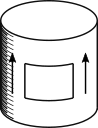
\includegraphics{img/statesAndMeasurements_00.png}
\caption{Apparatus}
\end{figure}

Before the apparatus interacts with (measures) the spin, the display is
blank. After it measures \(\sigma\), the display shows +1 or -1.

    \hypertarget{repeating-a-measurement}{%
\paragraph{Repeating a Measurement}\label{repeating-a-measurement}}

    Consider this simple experiment: point the apparatus in, say, the \(z\)
direction and measure the spin; then set the apparatus to neutral and
measure the same spin again; then repeat the process many times. If spin
was like any other classical property, we'd expect that the initial
result \(\sigma = +1\) would be followed by a sequence of
\(\sigma = +1\) , and similarly if we initially measured
\(\sigma = -1\). This hypothesis is drawn below.

\begin{figure}
\centering
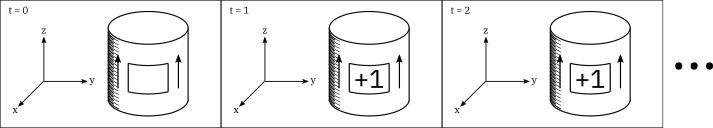
\includegraphics{img/statesAndMeasurements_01.png}
\caption{Experiment 1}
\end{figure}

    To see if our intuion is correct, we can run this experiment in
simulation using Qiskit. As we switch back and forth between speaking of
spins and our apparatus versus qubits and the Qiskit simulation, the
values of spin \{+1, -1\} which are natural for thinking about
orientation, are relabeled as the qubit states \{0, 1\} which are
natural for relating qubits to bits.

Before we can run the experiment, we need to first
\href{https://qiskit.org/documentation/install.html}{install Qiskit}.
Once it's installed, import it along with NumPy:

    \begin{Verbatim}[commandchars=\\\{\}]
{\color{incolor}In [{\color{incolor}1}]:} \PY{k+kn}{from} \PY{n+nn}{qiskit} \PY{k}{import} \PY{n}{QuantumCircuit}\PY{p}{,} \PY{n}{ClassicalRegister}\PY{p}{,} \PY{n}{QuantumRegister}\PY{p}{,} \PY{n}{execute}\PY{p}{,} \PY{n}{Aer}
        \PY{k+kn}{from} \PY{n+nn}{qiskit}\PY{n+nn}{.}\PY{n+nn}{tools}\PY{n+nn}{.}\PY{n+nn}{visualization} \PY{k}{import} \PY{n}{circuit\PYZus{}drawer}\PY{p}{,} \PY{n}{plot\PYZus{}histogram}
        \PY{k+kn}{import} \PY{n+nn}{numpy} \PY{k}{as} \PY{n+nn}{np}
        \PY{k+kn}{from} \PY{n+nn}{numpy} \PY{k}{import} \PY{n}{pi}
\end{Verbatim}


    The experiment can be described by a \texttt{QuantumCircuit} with a
single qubit (in a \texttt{QuantumRegister}) and as many bits (in a
\texttt{ClassicalRegister}) as we would like to store each measurement.

    \begin{Verbatim}[commandchars=\\\{\}]
{\color{incolor}In [{\color{incolor}2}]:} \PY{n}{num\PYZus{}measurements} \PY{o}{=} \PY{l+m+mi}{5}
        
        \PY{n}{q} \PY{o}{=} \PY{n}{QuantumRegister}\PY{p}{(}\PY{l+m+mi}{1}\PY{p}{)}
        \PY{n}{c} \PY{o}{=} \PY{n}{ClassicalRegister}\PY{p}{(}\PY{n}{num\PYZus{}measurements}\PY{p}{)}
        
        \PY{n}{circ} \PY{o}{=} \PY{n}{QuantumCircuit}\PY{p}{(}\PY{n}{q}\PY{p}{,}\PY{n}{c}\PY{p}{)}
        
        \PY{k}{for} \PY{n}{m} \PY{o+ow}{in} \PY{n+nb}{range}\PY{p}{(}\PY{n}{num\PYZus{}measurements}\PY{p}{)}\PY{p}{:}
            \PY{n}{circ}\PY{o}{.}\PY{n}{measure}\PY{p}{(}\PY{n}{q}\PY{p}{[}\PY{l+m+mi}{0}\PY{p}{]}\PY{p}{,}\PY{n}{c}\PY{p}{[}\PY{n}{m}\PY{p}{]}\PY{p}{)} 
        
        \PY{n}{circuit\PYZus{}drawer}\PY{p}{(}\PY{n}{circ}\PY{p}{,} \PY{n}{output}\PY{o}{=}\PY{l+s+s1}{\PYZsq{}}\PY{l+s+s1}{mpl}\PY{l+s+s1}{\PYZsq{}}\PY{p}{)}
\end{Verbatim}

\texttt{\color{outcolor}Out[{\color{outcolor}2}]:}
    
    \begin{center}
    \adjustimage{max size={0.9\linewidth}{0.9\paperheight}}{output_7_0.png}
    \end{center}
    { \hspace*{\fill} \\}
    

    Qiskit has several simulators in an included module called
\href{https://qiskit.org/aer}{Aer}. Since our simulation involves
measurements, we will use the simulator called \texttt{qasm\_simulator}.
Perform the simulation using \texttt{execute}, and specify that the
experiment is to be done only once by passing the parameter/value pair
\texttt{shots=1}.

    \begin{Verbatim}[commandchars=\\\{\}]
{\color{incolor}In [{\color{incolor}3}]:} \PY{n}{backend\PYZus{}sim} \PY{o}{=} \PY{n}{Aer}\PY{o}{.}\PY{n}{get\PYZus{}backend}\PY{p}{(}\PY{l+s+s1}{\PYZsq{}}\PY{l+s+s1}{qasm\PYZus{}simulator}\PY{l+s+s1}{\PYZsq{}}\PY{p}{)}
        
        \PY{n}{job\PYZus{}sim} \PY{o}{=} \PY{n}{execute}\PY{p}{(}\PY{n}{circ}\PY{p}{,} \PY{n}{backend\PYZus{}sim}\PY{p}{,} \PY{n}{shots}\PY{o}{=}\PY{l+m+mi}{1}\PY{p}{)}
        
        \PY{n}{result\PYZus{}sim} \PY{o}{=} \PY{n}{job\PYZus{}sim}\PY{o}{.}\PY{n}{result}\PY{p}{(}\PY{p}{)}
\end{Verbatim}


    You can access the result with the \texttt{get\_counts} function.

    \begin{Verbatim}[commandchars=\\\{\}]
{\color{incolor}In [{\color{incolor}4}]:} \PY{n}{counts} \PY{o}{=} \PY{n}{result\PYZus{}sim}\PY{o}{.}\PY{n}{get\PYZus{}counts}\PY{p}{(}\PY{n}{circ}\PY{p}{)}
        \PY{n+nb}{print}\PY{p}{(}\PY{n}{counts}\PY{p}{)}
\end{Verbatim}


    \begin{Verbatim}[commandchars=\\\{\}]
\{'00000': 1\}

    \end{Verbatim}

    The printed result is to be read from right to left, as you would extend
a binary number counting from zero. The number after the colon
(\texttt{:}) is the number of \texttt{shots} for which this result was
observed.

Our initial measurement of \(\sigma = +1\) (\(q = 0\)) was verified for
all subsequent measurements. We say that the apparatus \emph{prepares}
the spin in a state, and further measurements \emph{confirm} the state.

    \hypertarget{flipping-our-perspective}{%
\paragraph{Flipping Our Perspective}\label{flipping-our-perspective}}

    A simple change in the experiment will help reveal more of the spin's
spatial nature. Now, after preparing the spin (by measuring it with
\(A\)) we flip \(A\) upside down, then measure \(\sigma\) again. Our
classical intuition tells us that if we initially prepared
\(\sigma = +1\), then the flipped apparatus displays \(\sigma = -1\)
(and similarly if we prepared \(\sigma = -1\)). Our intuitive
expectation is drawn below.

\begin{figure}
\centering
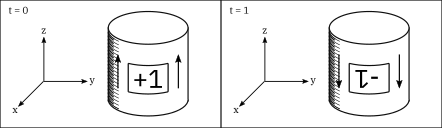
\includegraphics{img/statesAndMeasurements_02.png}
\caption{Experiment 2}
\end{figure}

Let's run the experiment in simulation. To flip the apparatus, we will
use a quantum circuit gate called the \(R_x\) gate, which we'll explain
in detail later. For now, it's enough to know that \(R_x\) rotates the
apparatus about the \(x\) axis. \emph{(In quantum circuits, we flip the
qubit with gates, not the circuit, but for now, let's shift our
perspective as we flip it.)}

    \begin{Verbatim}[commandchars=\\\{\}]
{\color{incolor}In [{\color{incolor}5}]:} \PY{n}{num\PYZus{}measurements} \PY{o}{=} \PY{l+m+mi}{5}
        
        \PY{n}{q} \PY{o}{=} \PY{n}{QuantumRegister}\PY{p}{(}\PY{l+m+mi}{1}\PY{p}{)}
        \PY{n}{c} \PY{o}{=} \PY{n}{ClassicalRegister}\PY{p}{(}\PY{n}{num\PYZus{}measurements}\PY{p}{)}
        
        \PY{n}{circ} \PY{o}{=} \PY{n}{QuantumCircuit}\PY{p}{(}\PY{n}{q}\PY{p}{,}\PY{n}{c}\PY{p}{)}
        
        \PY{k}{for} \PY{n}{m} \PY{o+ow}{in} \PY{n+nb}{range}\PY{p}{(}\PY{n}{num\PYZus{}measurements}\PY{p}{)}\PY{p}{:}
            \PY{n}{circ}\PY{o}{.}\PY{n}{measure}\PY{p}{(}\PY{n}{q}\PY{p}{[}\PY{l+m+mi}{0}\PY{p}{]}\PY{p}{,}\PY{n}{c}\PY{p}{[}\PY{n}{m}\PY{p}{]}\PY{p}{)}
            \PY{n}{circ}\PY{o}{.}\PY{n}{rx}\PY{p}{(}\PY{n}{pi}\PY{p}{,} \PY{n}{q}\PY{p}{[}\PY{l+m+mi}{0}\PY{p}{]}\PY{p}{)}
        
        \PY{n}{circuit\PYZus{}drawer}\PY{p}{(}\PY{n}{circ}\PY{p}{,} \PY{n}{output}\PY{o}{=}\PY{l+s+s1}{\PYZsq{}}\PY{l+s+s1}{mpl}\PY{l+s+s1}{\PYZsq{}}\PY{p}{)}
\end{Verbatim}

\texttt{\color{outcolor}Out[{\color{outcolor}5}]:}
    
    \begin{center}
    \adjustimage{max size={0.9\linewidth}{0.9\paperheight}}{output_15_0.png}
    \end{center}
    { \hspace*{\fill} \\}
    

    \begin{Verbatim}[commandchars=\\\{\}]
{\color{incolor}In [{\color{incolor}6}]:} \PY{n}{job\PYZus{}sim} \PY{o}{=} \PY{n}{execute}\PY{p}{(}\PY{n}{circ}\PY{p}{,} \PY{n}{backend\PYZus{}sim}\PY{p}{,} \PY{n}{shots}\PY{o}{=}\PY{l+m+mi}{1}\PY{p}{)}
        
        \PY{n}{result\PYZus{}sim} \PY{o}{=} \PY{n}{job\PYZus{}sim}\PY{o}{.}\PY{n}{result}\PY{p}{(}\PY{p}{)}
        
        \PY{n}{counts} \PY{o}{=} \PY{n}{result\PYZus{}sim}\PY{o}{.}\PY{n}{get\PYZus{}counts}\PY{p}{(}\PY{n}{circ}\PY{p}{)}
        \PY{n+nb}{print}\PY{p}{(}\PY{n}{counts}\PY{p}{)}
\end{Verbatim}


    \begin{Verbatim}[commandchars=\\\{\}]
\{'01010': 1\}

    \end{Verbatim}

    Rememer that qubit measurement values of \{0,1\} are labels for spin
measurement values of \{+1, -1\}. From the results of our simulation, we
see that every time we flip the apparatus, the spin's value flips sign.
This behavior shows that \(\sigma\) has an orientation in space. We
might be inclined to think that the spin is like a spatial vector with
components \(\sigma_x\), \(\sigma_y\), \(\sigma_z\). Let's consider
another experiment to explore this hypothesis.

    \hypertarget{lying-it-down}{%
\paragraph{Lying It Down}\label{lying-it-down}}

    Another simple change in the experiment will finally reveal the
counterintuitive quantum nature of spin. Now, after preparing a spin
with \(A\) pointed along the \(z\) axis, we rotate \(A\) through an
arbitrary angle, say \(\pi/2\) radians (90 degrees) about the \(x\) axis
to have \(A\) pointing along the \(y\) axis, then measure \(\sigma\)
again. This experiment is drawn below.

\begin{figure}
\centering
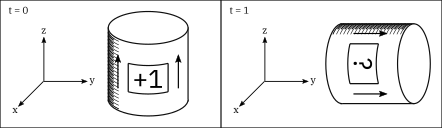
\includegraphics{img/statesAndMeasurements_03.png}
\caption{Experiment 3}
\end{figure}

If our hypothesis that \(\sigma\) is a spatial vector is correct, then
we'll have measured \(\sigma_z\), then \(\sigma_y\); if we prepared
\(\sigma_z = \pm 1\), then we should find that \(\sigma_y = 0\).

Let's run the experiment. To rotate the apparatus about the \(x\) axis,
we'll use the \(R_x\) quantum gate again.

    \begin{Verbatim}[commandchars=\\\{\}]
{\color{incolor}In [{\color{incolor}7}]:} \PY{n}{num\PYZus{}measurements} \PY{o}{=} \PY{l+m+mi}{1}
        
        \PY{n}{q} \PY{o}{=} \PY{n}{QuantumRegister}\PY{p}{(}\PY{l+m+mi}{1}\PY{p}{)}
        \PY{n}{c} \PY{o}{=} \PY{n}{ClassicalRegister}\PY{p}{(}\PY{n}{num\PYZus{}measurements}\PY{p}{)}
        
        \PY{n}{circ} \PY{o}{=} \PY{n}{QuantumCircuit}\PY{p}{(}\PY{n}{q}\PY{p}{,}\PY{n}{c}\PY{p}{)}
        
        \PY{n}{circ}\PY{o}{.}\PY{n}{rx}\PY{p}{(}\PY{n}{pi}\PY{o}{/}\PY{l+m+mi}{2}\PY{p}{,} \PY{n}{q}\PY{p}{)}
        \PY{n}{circ}\PY{o}{.}\PY{n}{measure}\PY{p}{(}\PY{n}{q}\PY{p}{,} \PY{n}{c}\PY{p}{)}
        
        \PY{n}{circuit\PYZus{}drawer}\PY{p}{(}\PY{n}{circ}\PY{p}{,} \PY{n}{output}\PY{o}{=}\PY{l+s+s1}{\PYZsq{}}\PY{l+s+s1}{mpl}\PY{l+s+s1}{\PYZsq{}}\PY{p}{)}
\end{Verbatim}

\texttt{\color{outcolor}Out[{\color{outcolor}7}]:}
    
    \begin{center}
    \adjustimage{max size={0.9\linewidth}{0.9\paperheight}}{output_20_0.png}
    \end{center}
    { \hspace*{\fill} \\}
    

    \begin{Verbatim}[commandchars=\\\{\}]
{\color{incolor}In [{\color{incolor}8}]:} \PY{n}{job\PYZus{}sim} \PY{o}{=} \PY{n}{execute}\PY{p}{(}\PY{n}{circ}\PY{p}{,} \PY{n}{backend\PYZus{}sim}\PY{p}{,} \PY{n}{shots}\PY{o}{=}\PY{l+m+mi}{1}\PY{p}{)}
        
        \PY{n}{result\PYZus{}sim} \PY{o}{=} \PY{n}{job\PYZus{}sim}\PY{o}{.}\PY{n}{result}\PY{p}{(}\PY{p}{)}
        
        \PY{n}{counts} \PY{o}{=} \PY{n}{result\PYZus{}sim}\PY{o}{.}\PY{n}{get\PYZus{}counts}\PY{p}{(}\PY{n}{circ}\PY{p}{)}
        \PY{n+nb}{print}\PY{p}{(}\PY{n}{counts}\PY{p}{)}
\end{Verbatim}


    \begin{Verbatim}[commandchars=\\\{\}]
\{'1': 1\}

    \end{Verbatim}

    The printed result shows that, counter to our intuition, we do
\textbf{not} find that \(\sigma_y = 0\) (\(q_y = 1/2\)). Instead, we
have found that the apparatus measures either \(\sigma_y = +1\) or
\(\sigma_y = -1\) (\(q_y = 0\) or \(q_y = 1\)). In fact, no matter which
way \(A\) is pointed, it only ever measures (displays)
\(\sigma = \pm 1\) (\(q = 0\) or \(q = 1\)).

    The second experiment showed that spin does have a spatial orientation,
but the third experiment revealed that it is not described well by a
spatial vector. Let's experiment further to get a better mathematical
understanding of the system.

The procedures of the first two experiments followed a simple pattern
when repeated in a series. Let's see what happens if we repeat the
procedure in the third experiment:

\begin{enumerate}
\def\labelenumi{\arabic{enumi}.}
\tightlist
\item
  Point \(A\) along the \(z\) axis.
\item
  Prepare \(\sigma = +1\).
\item
  Rotate \(A\) to point along the \(y\) axis.
\item
  Measure \(\sigma\).
\item
  Record the result.
\end{enumerate}

Intuitively, we'd expect each measurement to be consistent: verifying
the true, real state of the spin. Let's run the experiment to see if our
intution is confirmed.

    \begin{Verbatim}[commandchars=\\\{\}]
{\color{incolor}In [{\color{incolor}9}]:} \PY{n}{repetitions} \PY{o}{=} \PY{l+m+mi}{1024}
        
        \PY{n}{job\PYZus{}sim} \PY{o}{=} \PY{n}{execute}\PY{p}{(}\PY{n}{circ}\PY{p}{,} \PY{n}{backend\PYZus{}sim}\PY{p}{,} \PY{n}{shots}\PY{o}{=}\PY{n}{repetitions}\PY{p}{)}
        
        \PY{n}{result\PYZus{}sim} \PY{o}{=} \PY{n}{job\PYZus{}sim}\PY{o}{.}\PY{n}{result}\PY{p}{(}\PY{p}{)}
        
        \PY{n}{counts} \PY{o}{=} \PY{n}{result\PYZus{}sim}\PY{o}{.}\PY{n}{get\PYZus{}counts}\PY{p}{(}\PY{n}{circ}\PY{p}{)}
        \PY{n+nb}{print}\PY{p}{(}\PY{n}{counts}\PY{p}{)}
\end{Verbatim}


    \begin{Verbatim}[commandchars=\\\{\}]
\{'1': 511, '0': 513\}

    \end{Verbatim}

    The printed result shows the number of times each state was observed out
of the 1024 \texttt{shots} (repetitions) of our simulation. We can
visualize the results as a histogram:

    \begin{Verbatim}[commandchars=\\\{\}]
{\color{incolor}In [{\color{incolor}10}]:} \PY{n}{plot\PYZus{}histogram}\PY{p}{(}\PY{n}{counts}\PY{p}{)}
\end{Verbatim}

\texttt{\color{outcolor}Out[{\color{outcolor}10}]:}
    
    \begin{center}
    \adjustimage{max size={0.9\linewidth}{0.9\paperheight}}{output_26_0.png}
    \end{center}
    { \hspace*{\fill} \\}
    

    The repeated procedure has resulted in a random series of +1 and -1!
This is absolutely not consistent with our inuition of deterministic
reality if spin is a spatial vector. However, the result does not point
to total chaos. With enough repetitions, we'd find that the +1 and -1
events occur with equal frequency. In other words, the events have an
equal probability of occurrence with an average spin value of zero.

    We've found that the average of many repeated measurements is what we'd
intuitively (classically) expect of a spatial vector, although each
individual measurement is not. This is a conceptual bridge between our
classical expectations and quantum behavior. If the initial and final
orientations of the apparatus were other than along the \(z\) and \(y\)
axes, we would find the same result: an average value that agrees with
the classical intuition of spatial vectors, and individual random
measurements of +1 and -1 that run counter to the classical intuition.

    \hypertarget{testing-your-new-quantum-intuition}{%
\paragraph{Testing Your New Quantum
Intuition}\label{testing-your-new-quantum-intuition}}

    To test your new intuition, consider what would happen if we first
prepared \(\sigma = +1\) along the \(z\) axis, pointed \(A\) along the
\(y\) axis to make a measurement, then spun \(A\) back to its original
orientation. If we made another measurement along the \(z\) axis, would
we confirm the first result every time we ran this procedure?

The answer is\ldots{} no. Consider how this scenario is similar to the
third experiment.

In this scenario, the intermediate measurement along the \(y\) axis
leaves the spin in a random state prior the final measurement along the
\(z\) axis. The measuring of one component (\(\sigma_y\)) destroys
information about another component (\(\sigma_z\)). In general, any
interaction that is strong enough to measure an aspect of a quantum
system is necessarily strong enough to disrupt another aspect of that
system.

Even if you agree with the argument above, I strongly encourage you to
write your own Qiskit simulation of this experiment.

    \hypertarget{logical-propositions}{%
\subsubsection{Logical Propositions}\label{logical-propositions}}


    % Add a bibliography block to the postdoc
    
    
    
    \end{document}
